\chapter{Parallelism}

% Brett
\section{Flat Parallelism}
%TODO include a flat parallelism kernel somewhere
In this section, we will discuss how to write `flat' parallel code using Kokkos. 
Flat parallel code is code that does not use Kokkos' thread teams concept. This means
that flat parallel code does not make use of GPU shared memory, or intra-team reductions.
Flat parallel code does have access to an atomic fetch and add function, 
but this can have performance costs. These costs occur because atomic fetch and add can 
cause a bottleneck if too many threads
are trying to write to the same memory location. Therefore, we were limited to
writing \emph{flat} algorithms in which each thread knew its responsibility and did not
have to interact with other threads. In this section we will describe how to write
high performing kernels for both the CPU and GPU using this flat parallelism
technique. We will also describe some of its shortcomings and which other
non-flat parallel algorithms solve these issues.

Over the course of our project, we identified four main factors that affect
code's performance. These factors are: the thread count, the amount of work
each thread must do, memory access patterns, and how data is laid out in memory.
The first two factors (thread count and work per thread) are linked and are 
inversely proportional to one another. 

The thread count and work per thread are generally determined by how far you
decide to break down a problem. For example, in \\ \texttt{ContractFieldFieldScalar}, which performs
many matrix multiplications, a programmer could make each thread do one full matrix
multiplication. In this case, the thread count must be equal to the number of cells,
or matrix multiplications, that must be calculated. Figuring out the best way
to break down the responsibility of a single thread requires looking at the
expected problem size. 

Representative use cases for the example of
\texttt{ContractFieldFieldScalar} have from one thousand to tens of thousands of cells, with
matrix sizes between eight by eight and sixty-four by one hundred twenty-five. In this case, 
when writing code for the GPU, it
is best to break down the problem into the smallest possible pieces that avoid interaction, which corresponds
to one thread per output element in each output matrix. This is
because the goal is to minimize the amount of work per thread on the GPU, while still
avoiding thread interaction. 

The question always becomes: how many threads per contraction is optimal? 
As we can see from the dimensions described above, our total number of threads will 
be roughly 1,000 times our number of threads per contraction. Therefore, we would like
to have between a couple hundred and a thousand threads per contraction. 
This will ensure that the GPU is being saturated, which is a necessary condition for
high performance.
To reiterate Section~\ref{CPU-GPU}, we need to make sure that the GPU always has a 
\emph{minimum} of 15,000 threads being
spawned, with numbers in the 100,000-1,000,000 range being preferable.

When we combine this knowledge with the
goal of the threads not being required to interact or write to the same
memory location, we discover that the ideal number of threads per contraction we can use for flat parallelism
is always the same as the maximum number of threads we can use per contraction, because
this maximizes thread count and minimizes the work per thread. 
The maximum number of threads we can use is equal to of entries in the output tensor,
because if we go over that number, then the threads would need to interact to write
to the same output location.

Note that the
expected output tensor dimensions range from a single number (for any problem
that contains \texttt{DataData} in its name), to sixty-four squared (the largest practical value for
\texttt{numLeftFields} and \texttt{numRightFields}, which are the dimensions of the output matrix
for some problems). This range means that if we use flat parallelism for the \texttt{DataData} contractions,
we will only be spawning 1,000-10,000 threads on the GPU in the normal use cases,
which are below acceptable in terms of saturation. We can see the results of this effect in Figure~%TODO (slower than serial)

Now that the number of threads and their responsibility are known, the best
access patterns and data layouts must be calculated. As described earlier, the
best access patterns and data layouts for threads on the CPU are ones that
utilize the cache. This means that when using CPU, which corresponds to code written with \texttt{Kokkos::OpenMP},
we want a thread's next memory read to be next to its current memory read.
However, when using the GPU, which corresponds to code written with \texttt{Kokkos::Cuda}, a thread's memory read should
be adjecent to the reads of threads with nearby indices, as these threads will be in the same warp. 

These two memory access patterns are in direct conflict. To solve this problem, Kokkos
abstracts out the data layout by introducing a data structure called a View that encodes 
multidimensional arrays with custom memory layouts. The main layout parameters to a Kokkos View
are \texttt{LayoutLeft} and \texttt{LayoutRight}. In \texttt{LayoutLeft}, the left-most indices are
adjacent in memory, i.e., incrementing the left-most index by 1 moves to the next memory location.
The opposite is true for \texttt{LayoutRight}.
This means we can use \texttt{LayoutLeft} for one architecture, (i.e.
\texttt{Kokkos::Cuda}), and \texttt{LayoutRight} for the other (\texttt{Kokkos::OpenMP})
\footnote{In fact, if the memory layout for a view is not provided, Kokkos will default
to \texttt{LayoutLeft} on the GPU and \texttt{LayoutRight} on a CPU}. 

All that remains is to
figure out how to arrange the data, or which order to put the indices so that
one layout coalesces the memory while the other uses the cache. This is best
shown by an example; in \texttt{ContractFieldFieldScalar} there are inputs $A_{c, l, p}$
and $B_{c, r, p}$. Assuming we have a thread per output element in output
$C_{c, l, r}$, then we can have the inputs ordered as follows: $A_{c, l, p}$
and $B_{c, r, p}$. When using \texttt{Kokkos::OpenMP}, we will assume that the Views are \texttt{LayoutRight}, so
$A_{i, j, k}$ will be right next to $A_{i, j, k+1}$ in memory, while $A_{i, j,
k}$ will be very far from $A_{i+1, j, k}$ in memory. Each thread needs to do a
dot product of a row in $A$ with a column in $B$, so a thread needs to loop
through all of $p$ for the same value of $c$ and $l$ in $A$ and also loop
through all of $p$ for the same $c$ and $r$ in $B$. Notice however that all the
different values of $p$ in $A$ and $B$, where $c$, $l$, and $r$ are fixed, are
next to each other in memory, sicne we are using \texttt{LayoutRight}. This means that it will be cache friendly for any
thread. 

In contrast, for \texttt{Kokkos::Cuda}, the memory accesses must
be coalesced in the optimal case. 
This can be achieved by using the same data, but storing it in \texttt{LayoutLeft} Views
instead of \texttt{LayoutRight} views. In this case, $c$ values that differ by 1 are adjacent in memory.
Therefore, if thread $x$ is
responsible for calculating $C_{i, j, k}$, thread $x+1$ should responsible for
calculating $C_{i+1, j, k}$. In this manner, by changing our threading policy and 
the layout of our Views, our memory accesses are now coalesced, as desired. 

Finding the best way to lay out memory to optimize for both the CPU and GPU is
not too difficult. One good technique is to first find the best way for caching (CPU),
then imagine using the opposite layout (left or right) and seeing if there is
any way to coalesce the memory. This way one functor can be used, the data
layout can be easily changed, and the performance for both the CPU and GPU will
be high. Using this flat parallel technique we have received many good results,
an example of which can be seen in Figure~\ref{lst:ContractFieldFieldScalar
speedup over serial}, but there are some issues with flat parallelism.

It is important to find a way to arrange the indices of your data such that 
caching and coalescing can be achieved by chaning the layout of the view (as we just did).
If we had not laid out our indices as we did above, i.e. if $c$ were in the middle rahter 
than on the left, then it can be difficult, or even impossible to come up with a threading 
policy for each of CPU and GPU to match it. In this case, we are back to the scenario of 
writing different code for different architectures, but the whole goal of our project 
was to avoid doing so.

\begin{figure}[!ht]
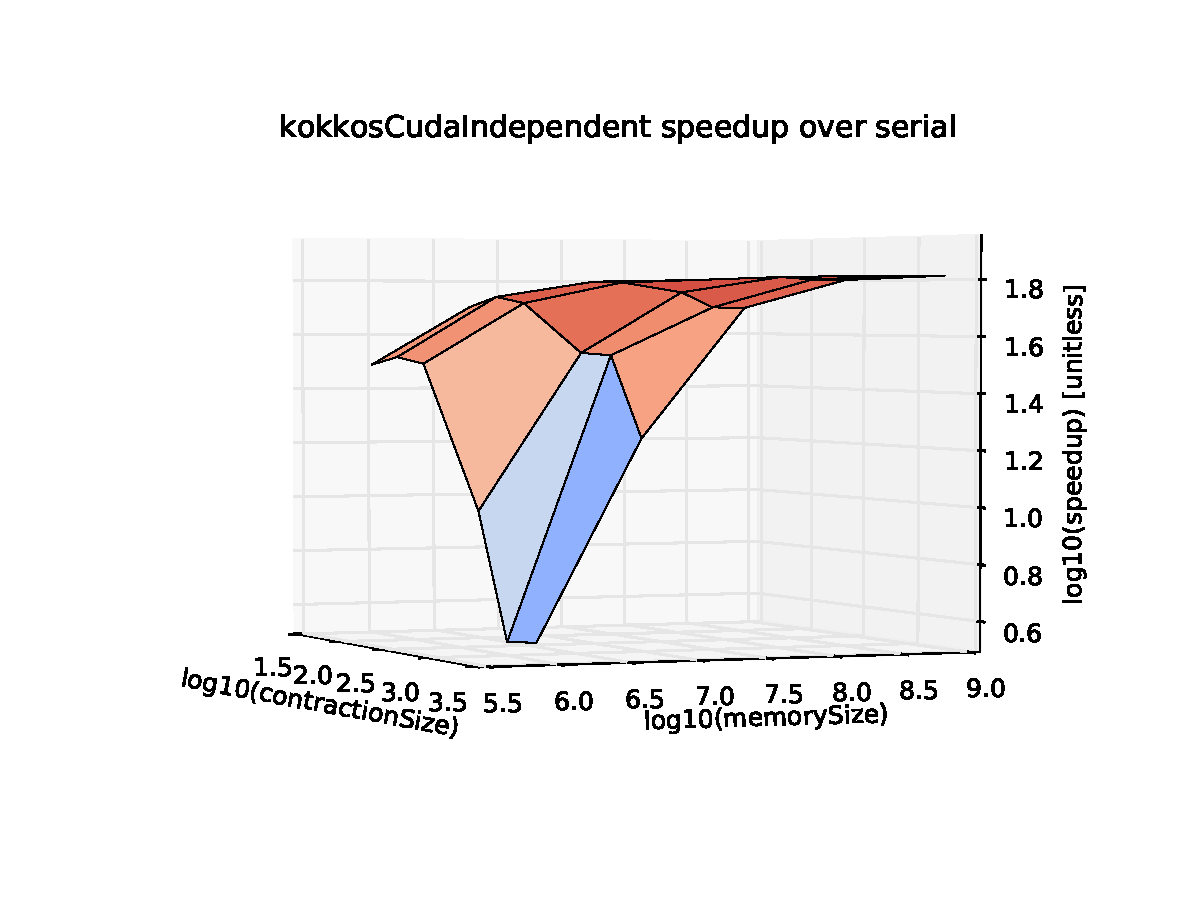
\includegraphics[scale=.8]{CFFS_VersusSerial_kokkosCudaIndependent.pdf}
\caption{Speedup over serial of the flat parallel algorithm of the
\texttt{ContractFieldFieldScalar} kernel. At its best this algorithm runs 60 times
faster than serial. The closest corner, where speedup is only about 4 times,
does not fit into Sandia's use case of expected problem sizes.
\label{lst:ContractFieldFieldScalar speedup over serial}} 
\end{figure}

Flat parallelism is an easy-to-implement, high-performing algorithm when there is 
enough work to saturate the GPU. However, there isn't always enough independent work to 
use flat parallelism. For example, on all the problems that have \texttt{DataData}
in their name, the output is simply an array of scalars, meaning that only one
thread per contraction can be used. The GPU is great for using tens of
thousands of threads to do computation, but when the number of threads is
severely limited, the CPU performs better, so other algorithms must be explored on the GPU. 
For examples of these algorithms, see Section~\ref{sec:reduction}

Another feature of the GPU that can be leveraged that is outside the scope of
flat parallelism is shared memory. Shared memory is essentially a user controlled cache
on the GPU. Algorithms that use shared memory will be discussed in
Section~\ref{slicing} and Section~\ref{sec:tiling}. The main benefits of not
using shared memory are it is easier to code and the speedup of shared memory over flat parallelism 
is relatively small compared to the speedup flat parallel algorithms reap over
serial code. 

% Ellen
\section{Reduction} \label{sec:reduction}
In some cases, flat parallelism can perform very poorly.  One problem with flat
parallelism is the potential lack of enough parallelism, as in
\texttt{ContractDataDataTensor}.  \texttt{ContractDataDataTensor} takes two
input arrays of three-dimensional tensors and produces an array of scalars.  See
Section~\ref{section:ContractDataDataTensor} for a more complete description of
this kernel.

The problem with the \texttt{DataData} class of tensor contractions (see
Table~\ref{tab:IntrepidNamingConvention}) is that they all output an array of
scalars -- that is, each individual contraction produces a scalar output.
Therefore, using flat parallelism, the greatest number of threads we can spawn
is one thread per contraction.  Each thread must then perform an entire
contraction independently, which in the case of
\texttt{ContractDataDataTensor}, means looping over all three of the
contraction indices.

Because of this, we see that when the contraction size is large and the memory
size is small -- when we cannot spawn enough threads to saturate the GPU and
each thread is responsible for a large amount of computation --
\texttt{ContractDataDataTensor} actually performs worse than serial.

A solution to this problem is to use a parallel reduction algorithm instead of
a flat parallelism algorithm.  In a reduction, multiple threads contribute to a
single output element.  This adds the necessary overhead of coordinating between
threads and combining their contributions, but allows more threads to be created
to saturate the GPU.

In Kokkos, threads can be organized into teams\footnote{for seasoned Cuda
programmers, teams correspond to Cuda blocks}.  Built-in reduction methods allow
teams to merge the contributions of their constituent threads.

Using this team-thread paradigm, we explored several methods of implementing
\texttt{ContractDataDataTensor} using a reduction algorithm.

\subsection{Team Depth 1}
    In this reduction algorithm, we assign one team per contraction, and each
    team has as many threads as there are elements in the \texttt{\_dim2}
    dimension.  Each thread therefore performs 
    $\texttt{\_numPoints} \times \texttt{\_dim2}$ multiplications, and then
    combines its local sum with that
    of the other threads in the team.


\begin{figure}[ht]
    \begin{lstlisting}[basicstyle=\tiny]
    // A team does one cell
    const unsigned int cellIndex = thread.league_rank();

    float sum = 0;
    
    // Each of the _dim2 threads contracts the qp and d1 dimensions.
    Kokkos::parallel_reduce(Kokkos::TeamThreadLoop(thread, _dim2),
    // We use an anonymous (lambda) function here:
    //      - [&] specifies that all automatic variables in the lambda are
    //         passed by reference; this allows us to save time that would be
    //         spent copying large arrays.
    //      - The lambda takes two arguments, d2 by value and localsum by
    //         reference.  The first argument is passed to each thread (this is
    //         the index into the _dim2 dimension to be looped over by this
    //         thread), and the second is the reduction target.
        [&] (const unsigned int d2, float& localsum) {
          for (unsigned int qp=0; qp < _numPoints; ++qp) {
            for (unsigned int d1=0; d1 < _dim1; ++d1) {
              // Each thread loops over two dimensions and then reduces into
              // localsum
              localsum +=  _leftInput(cellIndex, qp, d1, d2) *
                _rightInput(cellIndex, qp, d1, d2);
            }
          }
      }, sum);

    if (thread.team_rank() == 0) {
      _output(cellIndex) = sum;
    }
 \end{lstlisting}
\caption{Code from Team Depth 1 reduction functor for \texttt{ContractDataDataTensor}
\label{lst:ContractDataDataTensorDepth1Functor}} 
\end{figure}

\begin{figure}[ht]
    \begin{lstlisting}
    const team_policy reduction_policy(numCells, _dim2);
    Kokkos::parallel_for(reduction_policy, contractDataDataTensorTeamDepth1Functor );
    Kokkos::fence();
 \end{lstlisting}
\caption{Code from kernel launch for \texttt{ContractDataDataTensor} Team Depth
1 reduction
\label{lst:ContractDataDataTensorDepth1Call}} 
\end{figure}

In Figure~\ref{lst:ContractDataDataTensorDepth1Functor}, we can see that each
thread loops over the \texttt{\_numPoints} and \texttt{\_dim1} dimensions, and then
reduces with the other threads in the team.  The call to Kokkos'
\texttt{parallel\_for} function, seen in
Figure~\ref{lst:ContractDataDataTensorDepth1Call}, specifies an execution policy
in which the number of teams launched is \texttt{\_numCells}, and each team has
\texttt{\_dim2} threads.

\begin{figure}[ht]
    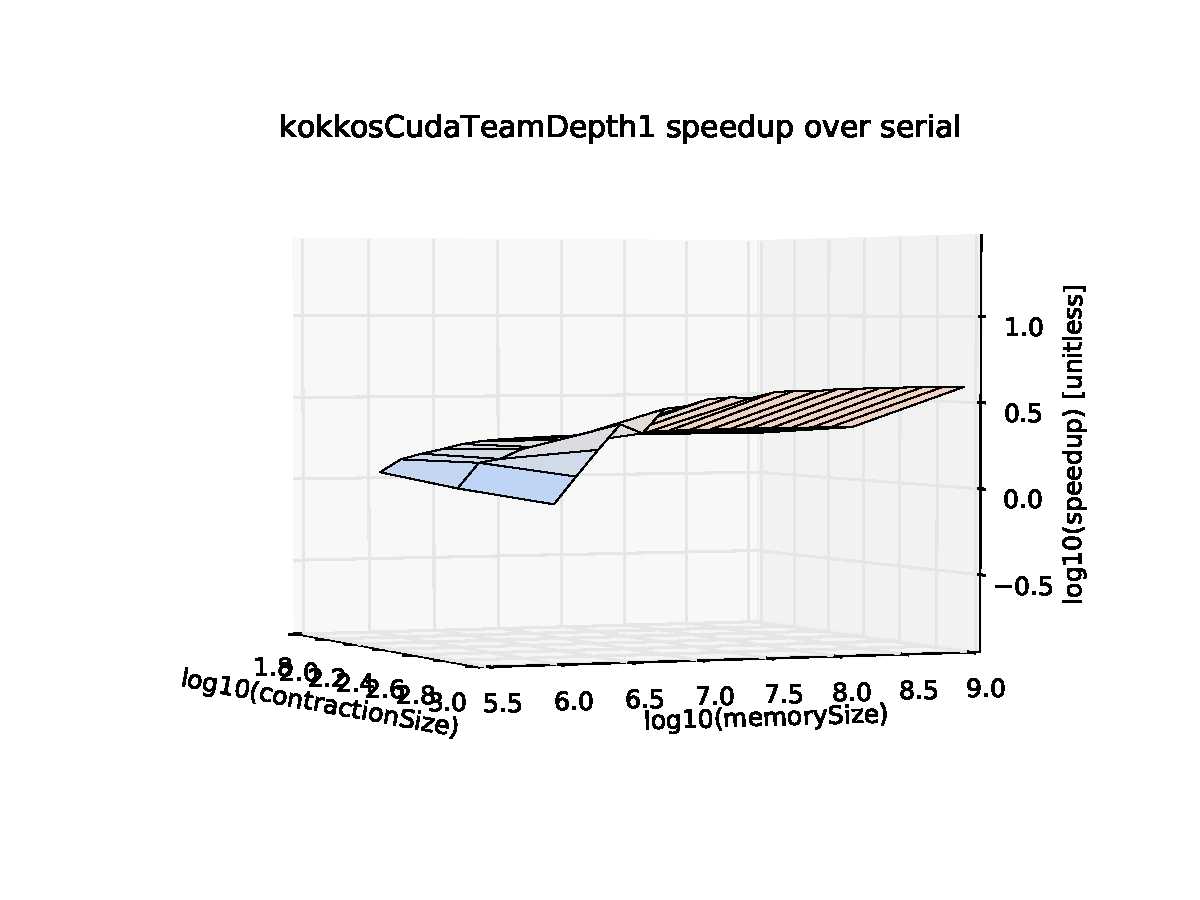
\includegraphics[scale=.55]{./VersusSerial_kokkosCudaTeamDepth1_clearCache_shadowfax.pdf}
\caption{Speedup of ContractDataDataTensor with Team Depth 1 algorithm over
    serial
\label{fig:ContractDataDataTensorDepth1}} 
\end{figure}

As shown in Figure~\ref{fig:ContractDataDataTensorDepth1}, this Team Depth 1
algorithm performs generally better than serial, but the speedup is minimal.
Therefore, we explored other reduction algorithms, which we hoped would yield
more impressive results.

\subsection{Team Depth 2}
    This reduction algorithm is similar to the previous one.  In a similar
    approach to that taken in the Team Depth 1 reduction, we assign one team per
    contraction.  In contrast to Team Depth 1, here each team has
    $\texttt{\_dim1} \times \texttt{\_dim2}$ threads, each responsible for
    \texttt{\_numPoints} multiplications.  Each thread then combines its local
    sum with that of the other threads in the team.

\begin{figure}[ht]
    \begin{lstlisting}
    // A team does one cell
    const unsigned int cellIndex = thread.league_rank();

    float sum = 0;
    // Each of the _dim1 * _dim2 threads contracts the _numPoints dimension
    Kokkos::parallel_reduce(Kokkos::TeamThreadLoop(thread, _dim1 * _dim2),
        [&] (const unsigned int threadIndex, float& localsum) {
          const unsigned int d1 = threadIndex / _dim2;
          const unsigned int d2 = threadIndex % _dim2;

          for (unsigned int qp = 0; qp < _numPoints; ++qp) {
            localsum +=  _leftInput(cellIndex, qp, d1, d2) *
              _rightInput(cellIndex, qp, d1, d2);
          }

      }, sum);

    if (thread.team_rank() == 0) {
      _output(cellIndex) = sum;
    }
    
 \end{lstlisting}
\caption{Code from Team Depth 2 reduction functor for \texttt{ContractDataDataTensor}
\label{lst:ContractDataDataTensorDepth2Functor}} 
\end{figure}

\begin{figure}[ht]
    \begin{lstlisting}
    const team_policy reduction_policy(numCells, _dim2 * _dim1);
    Kokkos::parallel_for(reduction_policy, contractDataDataTensorTeamDepth2Functor );
    Kokkos::fence();
 \end{lstlisting}
\caption{Code from kernel launch for \texttt{ContractDataDataTensor} Team Depth
2 reduction
\label{lst:ContractDataDataTensorDepth2Call}} 
\end{figure}

In Figure~\ref{lst:ContractDataDataTensorDepth2Functor}, we can see that each
thread loops over the \texttt{\_numPoints} dimension only, and then
reduces with the other threads in the team.  The call to Kokkos'
\texttt{parallel\_for} function, seen in
Figure~\ref{lst:ContractDataDataTensorDepth2Call}, specifies an execution policy
in which the number of teams launched is \texttt{\_numCells}, and each team has
$\texttt{\_dim1}\times \texttt{\_dim2}$ threads.

\begin{figure}[ht]
    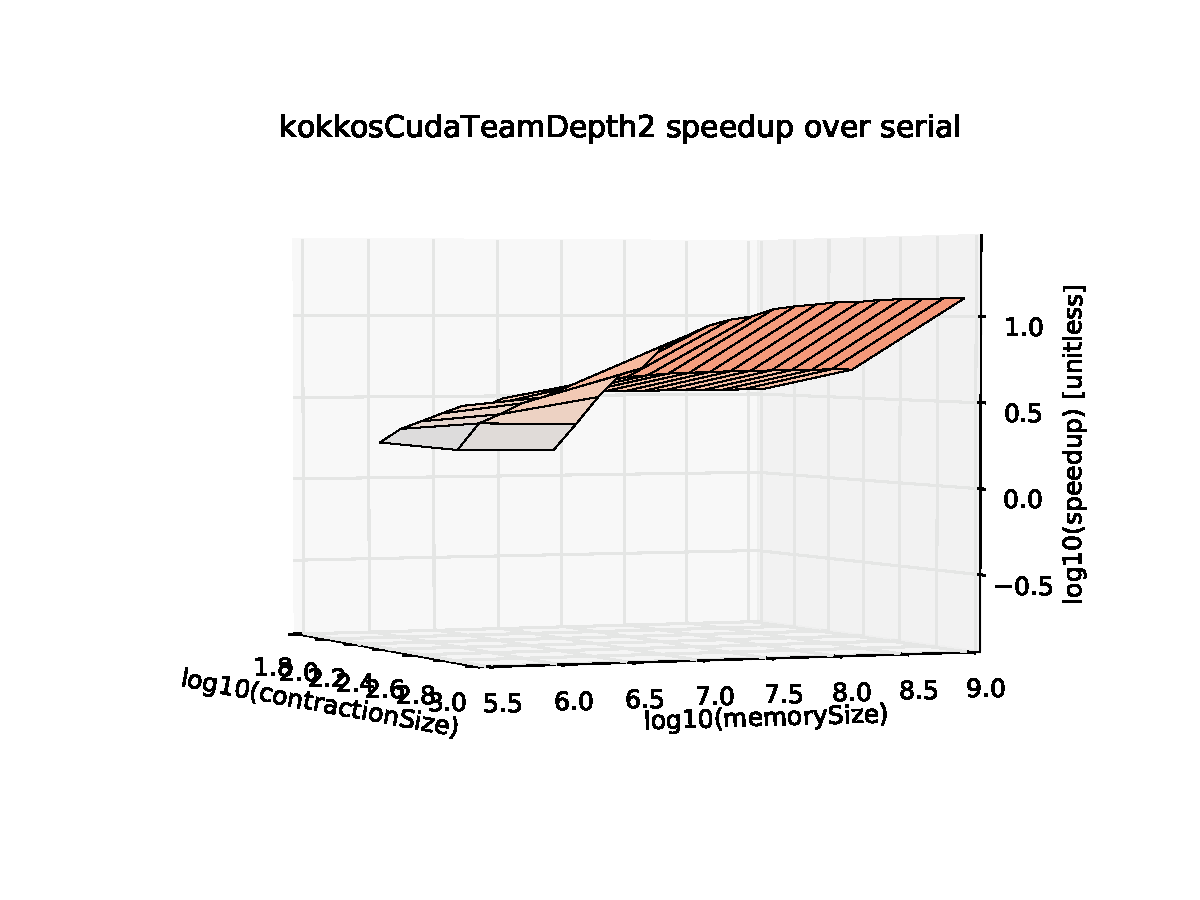
\includegraphics[scale=.55]{./VersusSerial_kokkosCudaTeamDepth2_clearCache_shadowfax.pdf}
\caption{Speedup of ContractDataDataTensor with Team Depth 2 algorithm over
    serial
\label{fig:ContractDataDataTensorDepth2}} 
\end{figure}

As shown in Figure~\ref{fig:ContractDataDataTensorDepth2}, this Team Depth 2
algorithm performs better than serial for the three representative use case..
In addition, the speedup is significant, and for large memory sizes, performs
nearly as well as the flat parallel algorithm.  Given the necessary overhead of
performing a reduction, we believe this to be a fairly good algorithm for good
performance across the
board.

However, because the team size is fixed based on the size of the \texttt{\_dim1}
and \texttt{\_dim2} dimensions, this algorithm may suffer performance penalties
or perhaps even bugs if these two dimensions are of unexpected sizes.  A more
generalizable algorithm therefore would be preferable.

\subsection{Teamstride}
    A more robust algorithm is one we call the Teamstride algorithm, in which
    each contraction is still assigned to a team, but a fixed number of threads
    are spawned for each team.  These threads treat the three contraction
    indices (\texttt{\_numPoints}, \texttt{\_dim1}, \texttt{\_dim2}) as if they were
    a single index, each thread striding forwards by the number of threads on
    this ``combined'' index.  This technique is similar to that used by OpenMP's
    collapse clause.  For instance, if this algorithm were run with a team size
    of sixty-four threads, then the zeroth thread in a team would sum the
    product of the zeroth elements, the sixty-fourth, the 128th, and so on.
    
\begin{figure}[ht]
    \begin{lstlisting}[basicstyle=\tiny]
    // A team does one cell
    const unsigned int cellIndex = thread.league_rank();

    float sum = 0;

    Kokkos::parallel_reduce (Kokkos::TeamThreadLoop(thread,cellSize),
       [&](const unsigned int threadIndex, float& localsum) {
        // Calculate the next element to add (striding by teamsize)
        const unsigned int qp = threadIndex / (_dim1 * _dim2);
        const unsigned int d1 = threadIndex % (_dim1 * _dim2) / _dim2;
        const unsigned int d2 = threadIndex % _dim2;
        
        localsum +=  _leftInput(cellIndex, qp, d1, d2) *
          _rightInput(cellIndex, qp, d1, d2);
      } , sum );

    if (thread.team_rank() == 0) {
      _output(cellIndex) = sum;
    }
\end{lstlisting}
\caption{Code from Teamstride functor for \texttt{ContractDataDataTensor}
\label{lst:ContractDataDataTensorTeamstrideFunctor}} 
\end{figure}

\begin{figure}[ht]
    \begin{lstlisting}[basicstyle=\tiny]
    const team_policy reduction_policy(numCells, 32);
    Kokkos::parallel_for( reduction_policy, contractDataDataTensorTeamstrideFunctor );
    Kokkos::fence();
    \end{lstlisting}
\caption{Code from kernel launch for \texttt{ContractDataDataTensor} Teamstride
\label{lst:ContractDataDataTensorTeamstrideCall}} 
\end{figure}

As seen in Figure~\ref{lst:ContractDataDataTensorTeamstrideFunctor}, this
algorithm requires more arithmetic on the part of each thread because the thread
is not responsible for looping over a single subset of indices but is instead
looping over all three contraction indices. The corresponding call in
Figure~\ref{lst:ContractDataDataTensorTeamstrideCall} uses a fixed team size of
32, unlike the previous two algorithms.  This team size seemed to be the best
for performance; a team size of 64 yielded similar speedup, but larger team
sizes did not perform as well.

\begin{figure}[ht]
    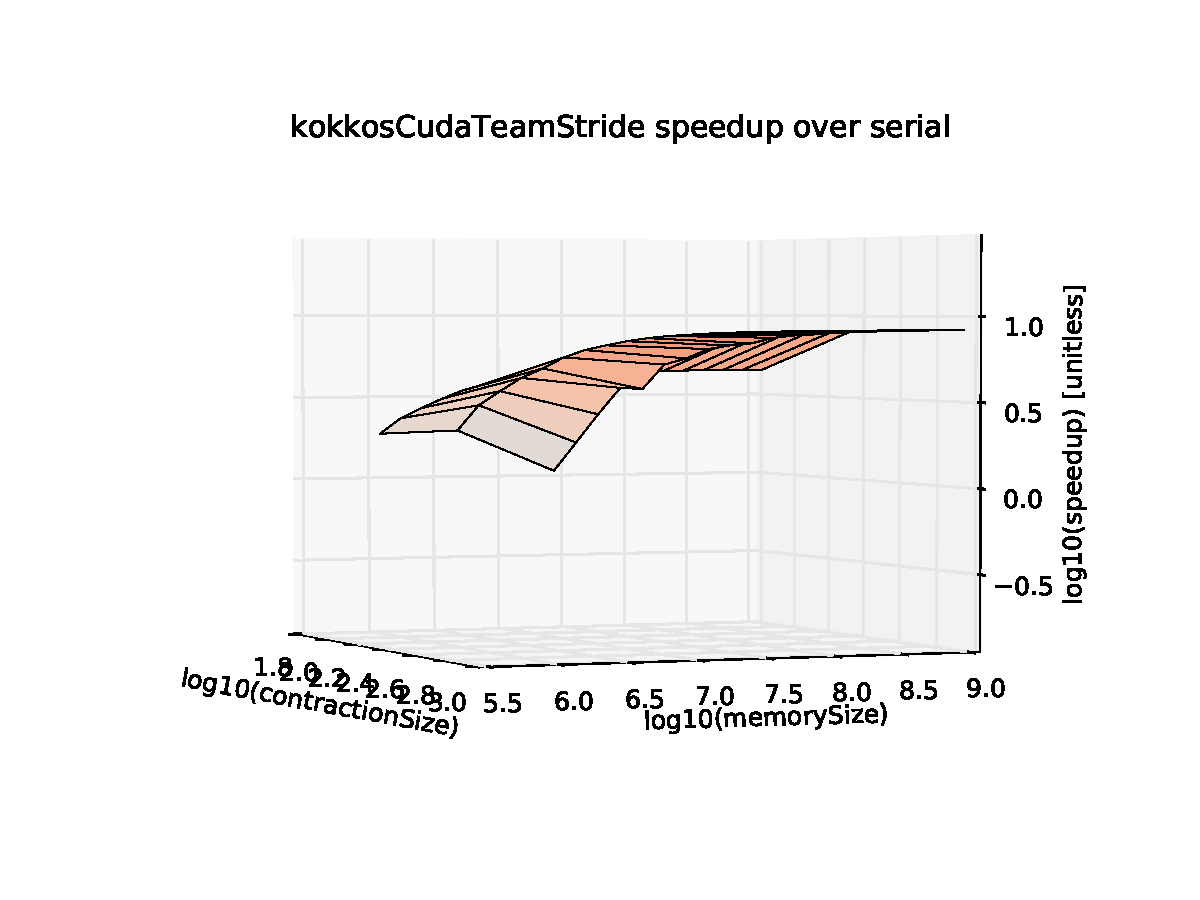
\includegraphics[scale=.55]{./VersusSerial_kokkosCudaTeamStride_clearCache_shadowfax.pdf}
\caption{Speedup of ContractDataDataTensor with Teamstride algorithm over
    serial
\label{fig:ContractDataDataTensorTeamstride}} 
\end{figure}

As shown in Figure~\ref{fig:ContractDataDataTensorTeamstride}, this algorithm
always performs better than serial.  Like with Team Depth 2, the speedup is
significant, and for large memory sizes, performs nearly as well as the flat
parallel algorithm.  In addition, this algorithm is more robust than Team Depth
2, since the number of threads per team is not determined by the size of the
input dimensions.  Therefore, the Teamstride reduction algorithm is likely the
most generalizable and performant variant of the reduction algorithms, and
should be explored in tensor contraction functions in which the inputs may
consist of a few large tensor contractions.

\subsection{Reduction Special Case}
As mentioned above, the parallel reduction algorithm outperforms the flat parallel algorithm when there is a small number of threads but lots of work per
thread. We also created parallel reduction algorithms for problems that did
not have this issue. An example is ContractFieldFieldScalar, which could have
as small as eight multiplies for a single thread since $p$ could be as few as
eight. As one may guess, the Teamstride parallel reduction algorithm performs worse than the flat
parallel algorithm. This is because we are creating more threads than necessary
and dividing up a small amount of work between at least 32 threads. The work is
divided between at least 32 threads because, remembering the architecture of
the GPU, there are 32 threads in a warp, all of which run in lock step. So in
cases where $p < 32$, threads are created that are not used in this reduction
algorithm. To mitigate this phenomenon we created a special reduction case.

The special reduction case creates fewer teams, giving more work per team, if
more than half of the threads in a warp are being wasted. Consider the
case of ContractFieldFieldScalar where 24 threads can wasted, because only 8
need to do a multiply then reduction, one quarter of the teams are created, and
each team is responsible for calculating four times as many outputs elements.
This case adds the code in
Figure~\ref{lst:ContractFieldFieldScalarReductionSpecialCase} to the functor's
operator() function. \\
\begin{figure}[!ht]
    \begin{lstlisting}
// Expects the Views to be LayoutRight so the memory is coalesced
// The if case is where the special reduction case is handled
if (numPoints <= 16) {	
	int myID = thread.league_rank()*(threadsPerTeam/numPoints)+thread.team_rank()/numPoints;
	int myMatrix = myID / (numLeftFields * numRightFields);
	int matrixIndex = myID - (myMatrix * (numLeftFields * numRightFields));
	int matrixRow = matrixIndex / numRightFields;
	int matrixCol = matrixIndex - (matrixRow * numRightFields);

	int pointIndex = thread.team_rank() % numPoints;

	float mult = leftView(myMatrix, matrixRow, pointIndex) 
		* rightView(myMatrix, pointIndex, matrixCol);

	Kokkos::atomic_fetch_add(&outputView(myMatrix, matrixRow, matrixCol), mult);
}
// This is where the normal reduction case is handled
else {
	int myID = thread.league_rank();
	int myMatrix = myID / (_numLeftFields * _numRightFields);
	int matrixIndex = myID - (myMatrix * (_numLeftFields * _numRightFields));
	int matrixRow = matrixIndex / _numRightFields;
	int matrixCol = matrixIndex - (matrixRow * _numRightFields);

	Kokkos::parallel_reduce(Kokkos::TeamThreadLoop(thread, _numPoints),
		[&] (const unsigned int& i, float& localSum) {
			localSum += _leftView(myMatrix, matrixRow, i) *
				_rightView(myMatrix, i, matrixCol);
			},
			sum);
	if (thread.team_rank() == 0) {
		_outputView(myMatrix, matrixRow, matrixCol) = sum;
	}
}
    \end{lstlisting}
\caption{Code for the special reduction case in \texttt{ContractFieldFieldScalar}
\label{lst:ContractFieldFieldScalarReductionSpecialCase}} 
\end{figure}

In the code of Figure~\ref{lst:ContractFieldFieldScalarReductionSpecialCase}, the number of multiplies, that is need is numPoints. If that number is less than 16, then we want one team to do more than one output. Increasing the number of active threads per team leads to higher efficiency and speed.
One thing that needs to be noted for the code in the special case is that an
\texttt{atomic\_fetch\_add} is used instead of a \texttt{parallel\_reduce}. This is due to the fact
that there is no \texttt{team\_reduce} function where half the threads reduce to one
location while the other half reduce to another location. This has the side
effect of requiring the output locations to be 0 before the calculation, while
in the "normal" reduction algorithm that is not necessary. 

Another point that needs to be reiterated is that this special case can still
perform worse than the flat parallel algorithm, but its purpose is to increase
the performance of a pure reduction algorithm in the region of the plot where it performs most poorly. Figure~\ref{CFFSTeamReduceSpecialCaseGraph} shows the effect of using the
special case. The flap up for small contraction sizes does not
exist for the algorithm not including the special case. The reduction with the special case outperforms the reduction algorithm without the special case by a lot for 
small contraction sizes.

\begin{figure}
    \centering
    \subfloat[][Here is a graph showing the special case of Team Reduction algorithm's speedup over serial for ContractFieldFieldScalar. The faster speeds for the smaller contraction size (far left) is where the special case is used.]{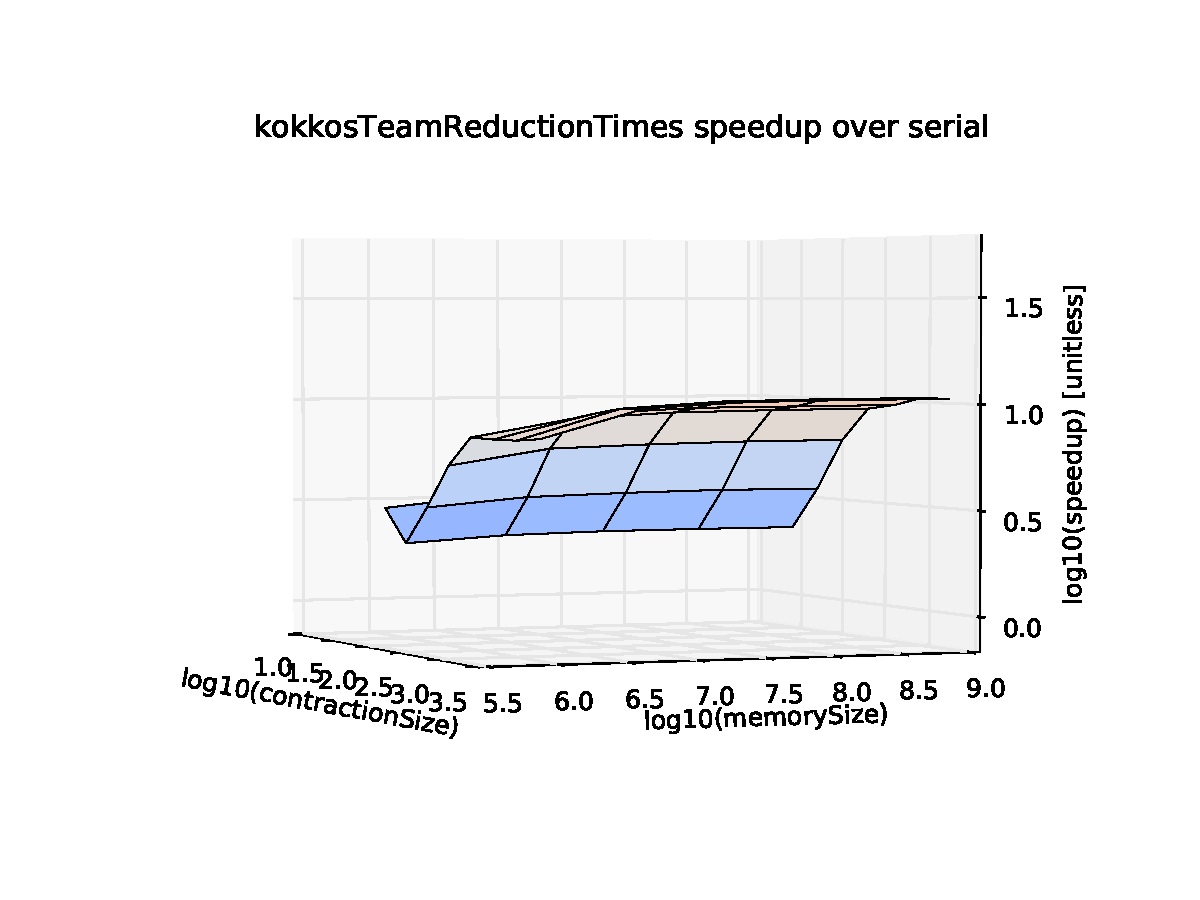
\includegraphics[scale = .30]{kokkosCFFSTeamReductionSpecialCase.pdf}
	\label{fig:CFFSSpecialReduction}}
	\:
	\subfloat[][ContractFieldFieldScalar team reduction's speedup over serial without the special case in the reduction. Notice that the smaller contraction sizes continue to perform worse, which was not the case for the reduction algorithm with the special case.]{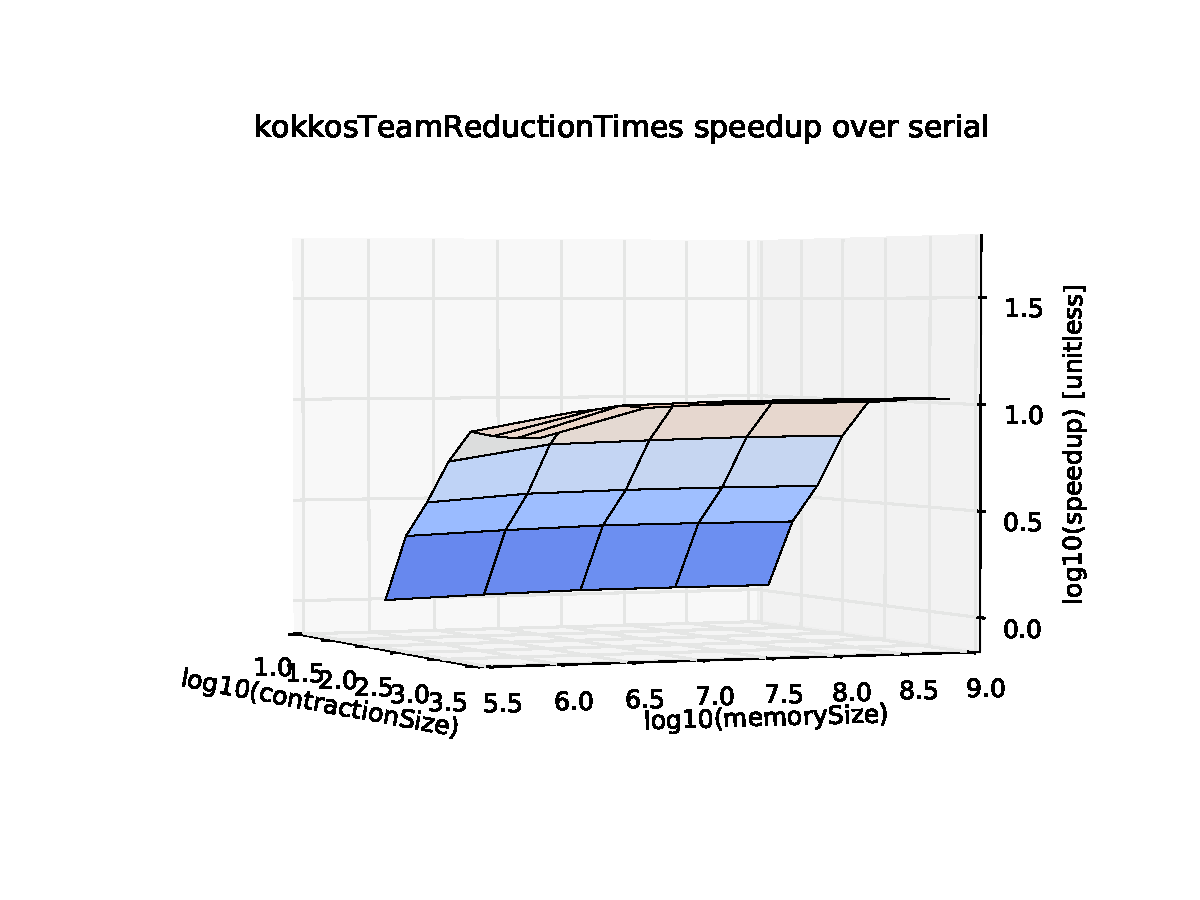
\includegraphics[scale = .3]{kokkosCFFSTeamReductionNoSpecialCase}
	\label{fig:CFFSWithoutSpecialReduction}}
    \caption{A comparison between the reduction algorithm with the special case and the reduction algorithm without the special case.}
\label{CFFSTeamReduceSpecialCaseGraph}
\end{figure}

%\begin{figure}[!ht] 
%    \centering
%    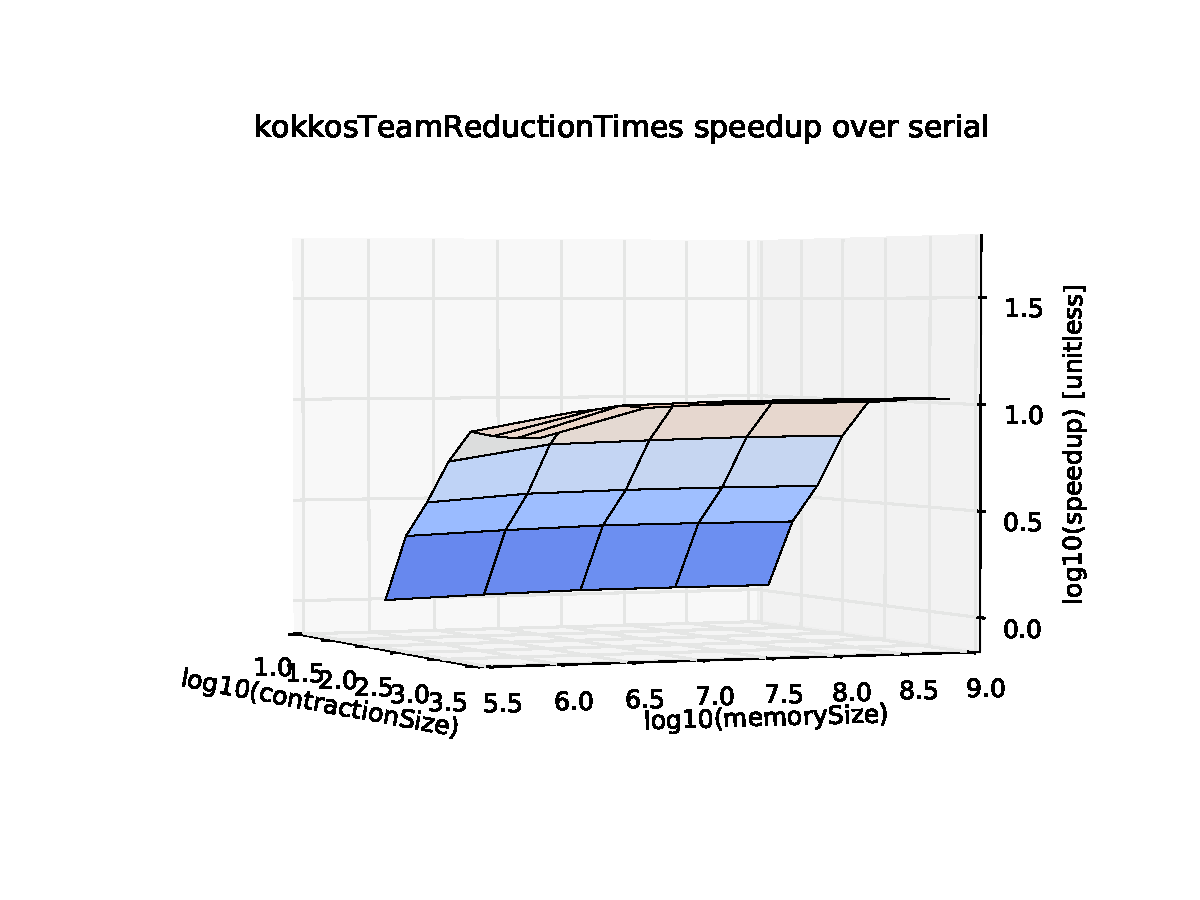
\includegraphics[scale = .8]{kokkosCFFSTeamReductionNoSpecialCase}
%    \caption{ContractFieldFieldScalar team reduction's speedup over serial without the special case in the reduction. %Notice that the smaller contraction sizes continue to perform worse, which was not the case for the reduction algorithm %with the special case.}
%\label{CFFSTeamReduceNoSpecialCaseGraph}
%\end{figure}


% Alex
\section{Slicing} \label{slicing}
Another general method we used for these contractions was slicing. The first
step of this method is to load one full contraction from the left input tensor into
shared memory. Then, we simultaneously computed every output element that was
dependent on that contraction as input. The clearest way to explain the
algorithm is by example. Consider one of the matrix multiplications in
\texttt{ContractFieldFieldScalar}. 

\begin{figure}
    \centering
    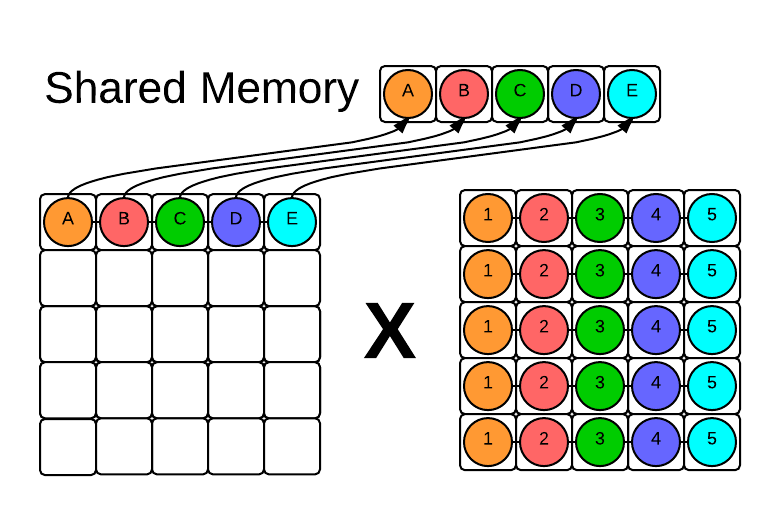
\includegraphics[scale = .55]{ContractFieldFieldScalarGraphic}
    \caption{Demonstration of memory accesses for a slicing implementation of ContractFieldFieldScalar}
\label{fig:Slicing}
\end{figure}

    In Figure~\ref{fig:Slicing}, on the left, we have the first of the two input matrices, whose first row's
elements are labeled $A-E$. On the right we have the second of the two inputs.
For the sake of simplicity, assume that we have one block of five threads which
are labeled by color. Each of the threads reads in one of the elements on the
right and copies it into shared memory. In cases where the number of elements
per contraction (row on the left) is unequal to the number of contractions
(columns on the right), we set the number of threads per block equal to the
number of contractions. This causes threads to either sit idle or loop multiple
times when reading the elements on the left into shared memory, but this is
clearly more efficient than forcing threads to compute more than one element.
	
    After the values of the contraction have been read into shared memory, we
have each thread compute the output element corresponding to one contraction.
This is shown on the right by the colored columns. Each thread reads every
element from shared memory and computes the contraction by multiplying these
elements with the columns of the right matrix. We see that throughout this
progress, memory accesses will be coalesced within the block, since each thread
reads the same element from shared memory then multiplies by an element that is
adjacent to the other elements the rest of the block is reading at that time. 
	
    For every other block of threads, the approach is similar, if Figure~\ref{fig:Slicing}
represents the first block of the contraction, then the second block will be
represented in Figure~\ref{fig:Slicing2}. 

\begin{figure}[b]
    \centering
    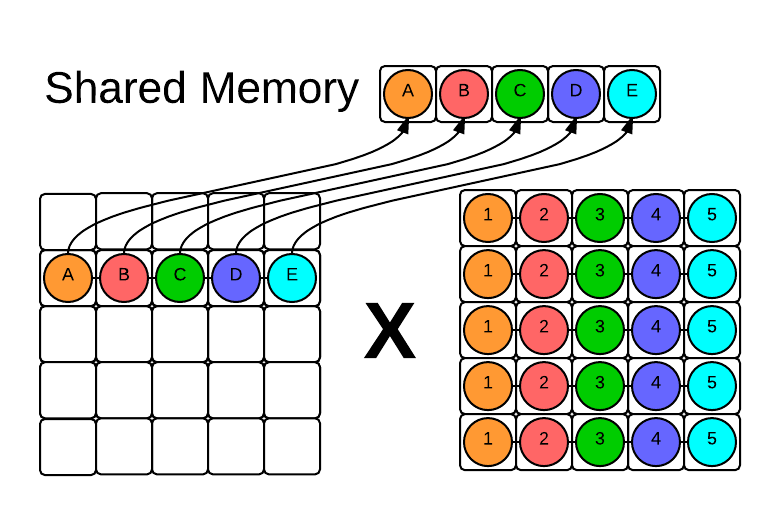
\includegraphics[scale = .55]{ContractFieldFieldScalarGraphic2}
    \caption{Demonstration of memory accesses for the second block of a slicing implementation of ContractFieldFieldScalar}
\label{fig:Slicing2}
\end{figure}

We see that for the FieldFieldScalar example, where our equation is given by
$L_{C,\ell,P} \times R_{C, \mathcal{R}, P} = O_{C,\ell, \mathcal{R}}$, the
number of blocks initialized by the algorithm will be equal $\ell \times C$,
since there are $\ell$ blocks per matrix, and we have $C$ matrices.
Additionally, there will be $\mathcal{R}$ threads per block. 

%TODO make this kokkos code?
    Cuda code for executing the algorithm as described above is included in Figure~\ref{lst:ContractFieldFieldScalarSlice},
although it has been simplified for clarity. 

\begin{figure}[ht]
    \begin{lstlisting} [basicstyle=\tiny]
     extern __shared__ float sliceStorage[];
     const unsigned int col = threadIdx.x;
     unsigned int currentBlock = blockIdx.x;
     unsigned int numBlocks = numBasis*numCells;
     
     syncthreads();
     const unsigned int cell = currentBlock / numBasis;
     const unsigned int row = currentBlock - cell * numBasis;

     for (unsigned int p = threadIdx.x; p < contractionSize; p += blockDim.x) {
        sliceStorage[p] = dev_contractionData_Left[cell*numBasis*contractionSize + row*contractionSize + p];
     }
     syncthreads();

     float sum = 0;
     for (int p = 0; p < contractionSize; ++p) {
       sum += sliceStorage[p] * dev_contractionData_Right[cell*numBasis*contractionSize +
        p*numBasis + col];
     }

     dev_contractionResults[cell*numBasis*numBasis + row*numBasis + col] = sum;
 \end{lstlisting}
\caption{Code from slicing algorithm on \texttt{ContractFieldFieldScalar}
\label{lst:ContractFieldFieldScalarSlice}} 
\end{figure}

    The main advantage of this approach is that it is easily generalizable to
tensor contractions of higher dimensions. Unlike tiling (described in Section~\ref{sec:tiling}), which is significantly
less intuitive in higher dimensions, it is easy to implement slicing in higher
dimensions by loading a larger slice into shared memory. Because of its
reliance on shared memory, there are many use cases in which we would expect
slicing to perform poorly. 

Intuitively, slicing is reliant on large contraction
sizes to produce speedup because in situations where the number of threads per
block is low it is unable to saturate the GPU. While this problem can be
remedied by increasing the number of contractions per block, it can introduce
problems with shared memory. Since shared memory is limited by nature, slicing
has to balance the amount of work per block with the amount of shared memory
available to that block.
	
    In situations where the problem has an inherently large amount of reuse
like \texttt{ContractFieldFieldScalar}, this problem can be remedied to some degree, but
in contractions without this feature, like \texttt{ContractDataDataScalar}, it seems
clear that slicing will not be an efficient algorithm. 
	
When we compare slicing approaches using one contraction per block to
independent flat parallelism on promising problems, we get underwhelming
results. 

%TODO make this a figure and ref it above
    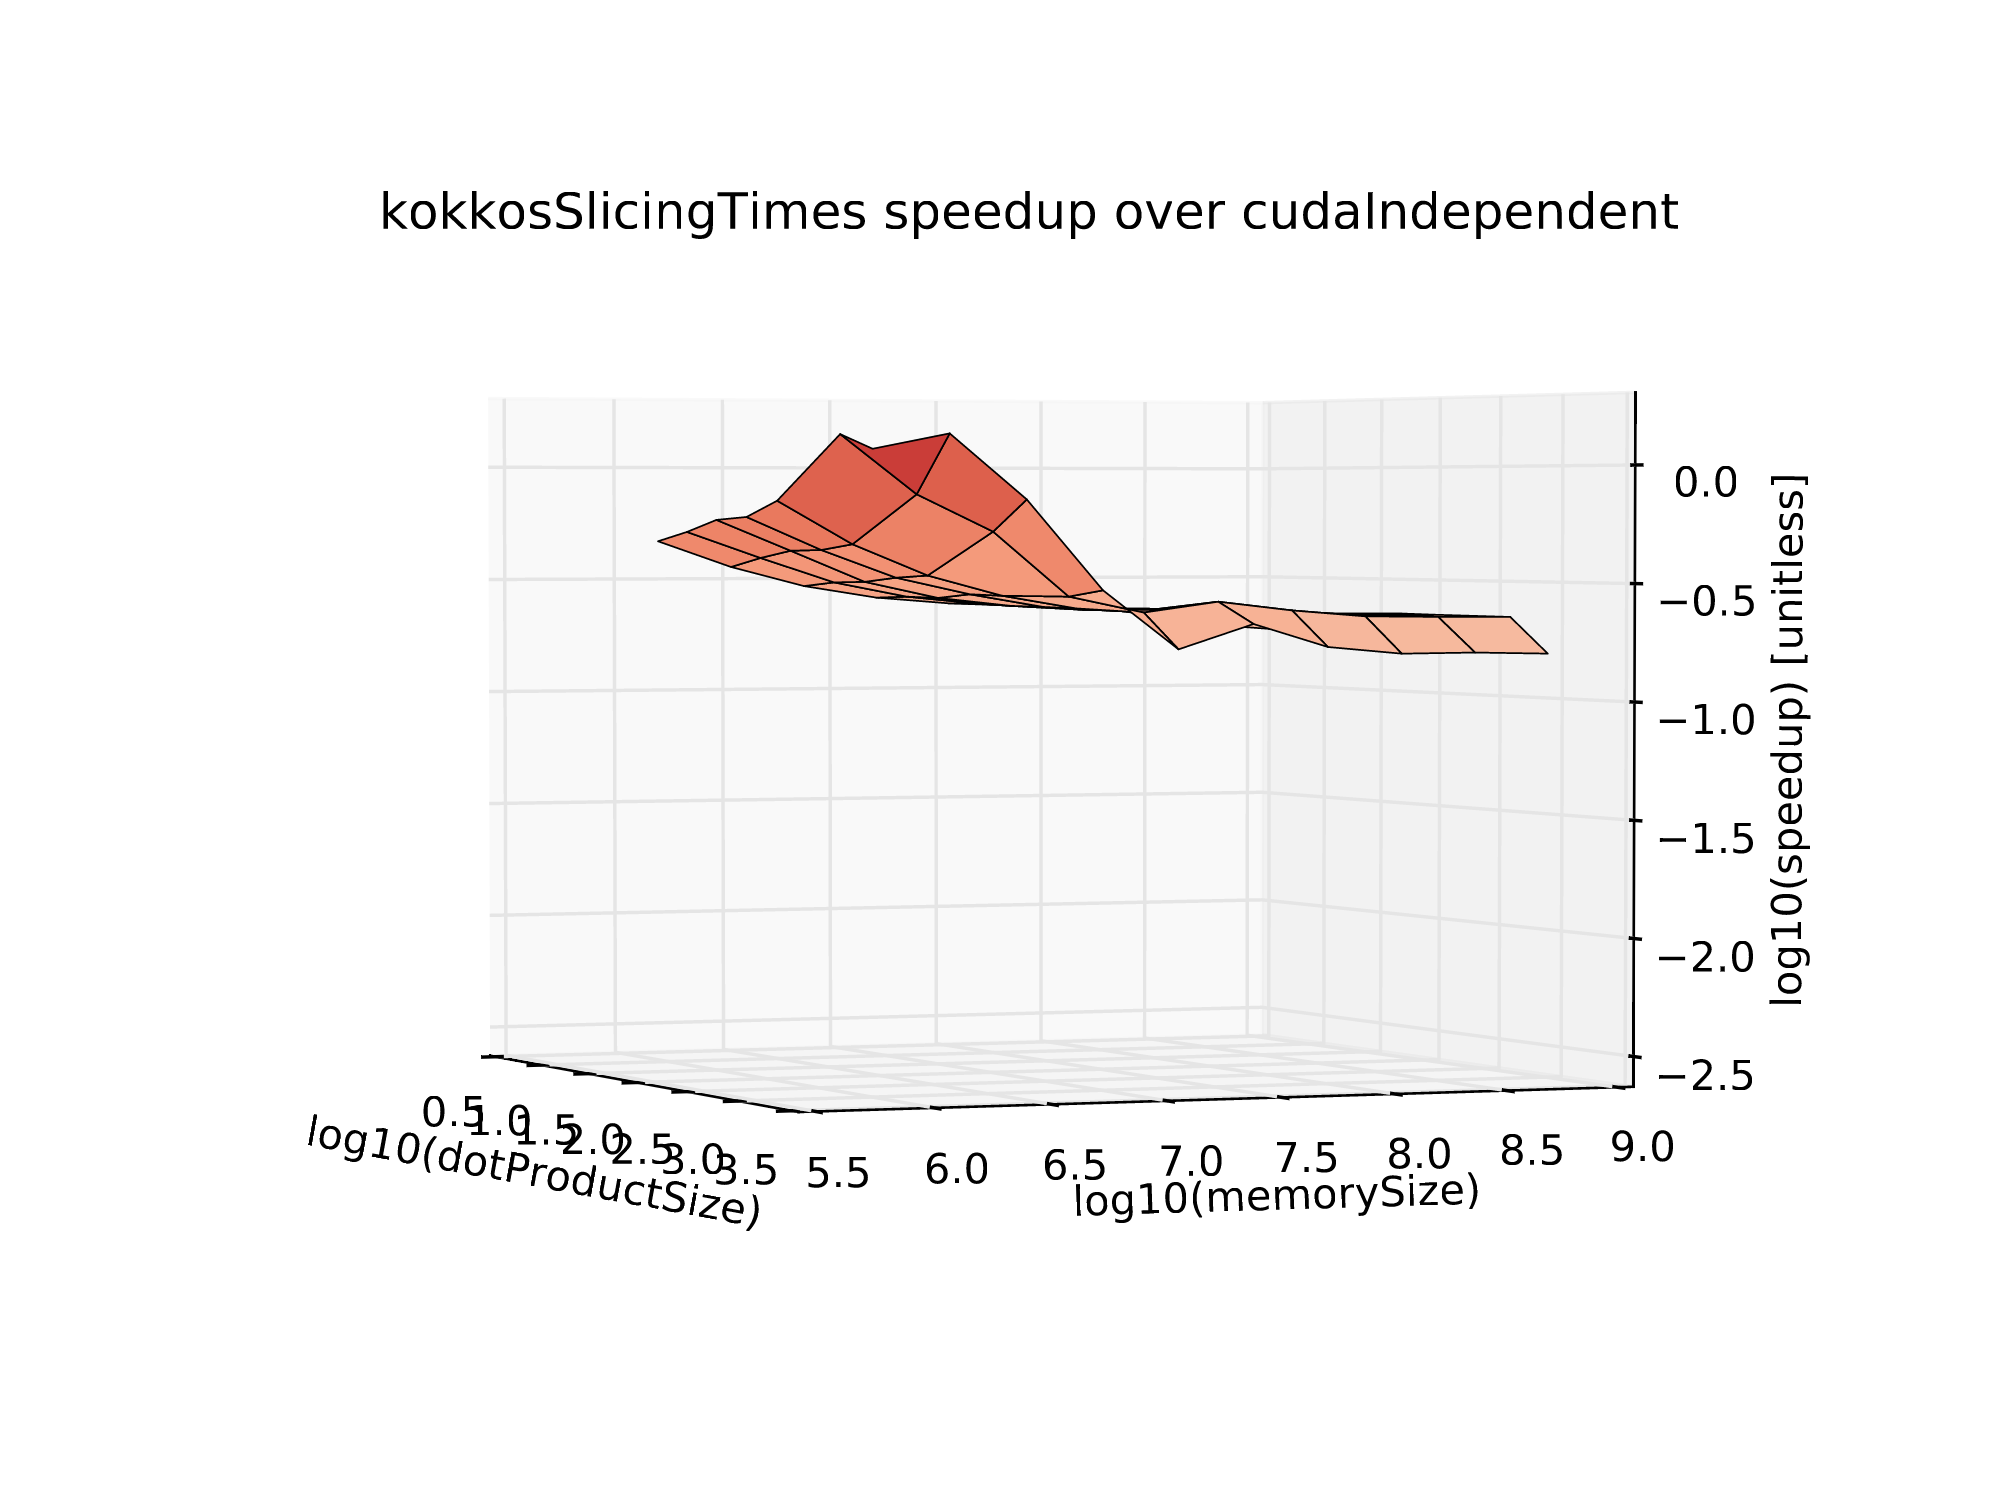
\includegraphics[scale = .17]{slicingvsindependent}

These results were generated by comparing independent algorithms to slicing on
\texttt{ContractFieldFieldScalar} with $\ell = \mathcal{R} = 10$ and $P \in [8,1024]$. We see
that in the corner where the memory size is small and contraction size is small
we get a small amount of speedup relative to flat Cuda code, which is
promising. This is the corner where we would expect slicing to perform the best
with respect to independent parallelism, since in this corner flat parallelism
is unable to fully saturate the GPU. The benefits of reuse in this corner are
significant enough to out-compete flat parallelism. On the rest of the graph,
however, the inability of slicing to saturate the GPU means that it is
significantly slower that flat parallelism. Since $\ell = \mathcal{R} = 10$,
the algorithm naturally only spawns 10 threads per block, which is not enough
to produce good results. 

Fortunately, this can be counteracted to some degree by loading multiple slices 
into shared memory simultaneously. This places a larger strain on shared memory, 
but also presents additional opportunities for parallelism. 
This technique has shown promising results on \texttt{ContractFieldFieldTensor}, as shown in Figure~(TODO) %TODO get this figure: 

%TODO {send help - I don't understand the python graph making code}

This shows that the adaptive slicing approach does have some process in these applications. These results were generated by loading two slices simultaneously in \texttt{ContractFieldFieldTensor} with $\ell = \mathcal{R} = 125$, $d_1 = d_2 = 4$, and $p=216$.

% Alex
\section{Tiling}\label{sec:tiling}

The final parallelization technique we used for these tensor contractions was
tiling. This technique is similar to the tiled technique for matrix
multiplication used in serial operations. Instead of relying on the cache to
retain the relevant pieces of information, however, we use shared memory to
explicitly store the data we care about. Once again, we will explain this
algorithm by example. Consider one of the matrix multiplications in
\texttt{ContractFieldFieldScalar} as shown in Figure~\ref{fig:Tiling}. 

%TODO replace this figure with the one from the poster
\begin{figure}[ht]
    \centering
    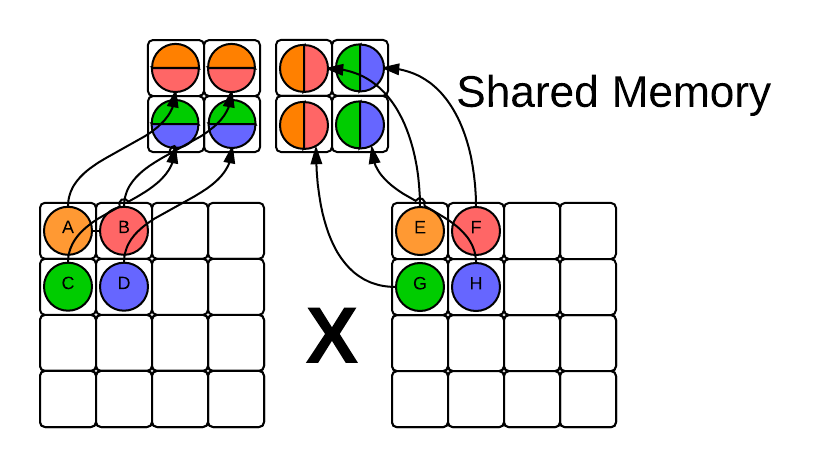
\includegraphics[scale = .7]{ContractFieldFieldScalarGraphicTiling}
    \caption{Demonstration of memory accesses for a tiling implementation of ContractFieldFieldScalar}
\label{fig:Tiling}
\end{figure}

For the sake of simplicity we'll consider a block to be four threads, which
simplifies our computation since the matrix is four by four. On the left hand
side, the block loads a four element tile into the shared memory of the
threads. Once these elements are loaded into memory, each thread can begin
computation of their element in the output matrix. Each thread computes as much
of their output element as they can using the elements in shared memory, then
we load a new tile into shared memory and continue the process, as shown in Figure~\ref{fig:Tiling2}.
We see that in this case we will have to load two tiles into shared memory
before we have computed every output element in the first tile in its entirety. 

%TODO replace this figure as well
\begin{figure}[ht]
    \centering
    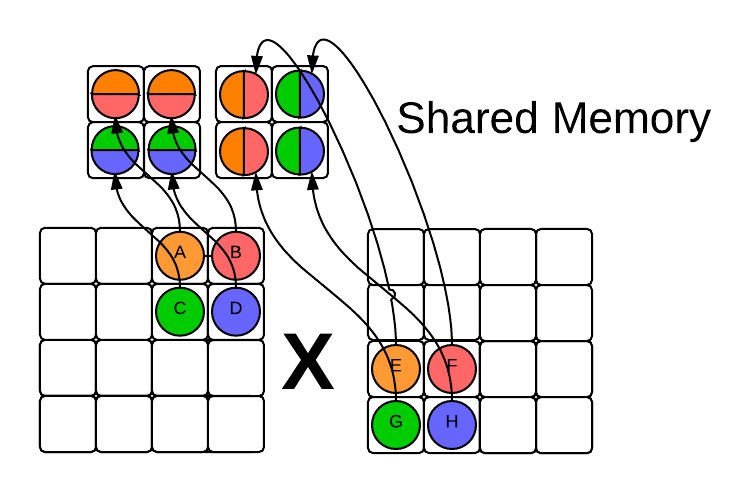
\includegraphics[scale = .7]{ContractFieldFieldScalarGraphicTiling2}
    \caption{Demonstration of memory accesses for a tiling implementation of ContractFieldFieldScalar}
\label{fig:Tiling2}
\end{figure}

    Tiling can be viewed as a more specialized version of slicing, since they
both use similar access patterns for shared memory. The difference between the
two lies in tiling's usage of multiple contractions per block, as well as the
the distribution of a contractions operations over multiple loops of the
routine. Because of these differences, tiling can routinely saturate the GPU in
a way that pure slicing cannot, since the algorithm inherently limits the
shared memory usage per block by reusing the same shared memory multiple times.
Additionally, if we set the dimension of our tiles intelligently, we can
reliably saturate the GPU with both blocks and threads, something that is very
difficult to do adaptively with pure slicing. 
	
%TODO this should probably be Kokkos, and not have the limitations
    Excerpts from our Cuda implementation of tiling are included below. The
code assumes that \texttt{tileSize} (the horizontal and vertical dimensions of a tile)
evenly divides both the contraction size and $\ell = \mathcal{R} =
\text{numBasis}$.
	
\begin{figure}[H]
    \begin{lstlisting} [basicstyle=\tiny]
  extern __shared__ float tileStorage[];
  const unsigned int numbersPerTile = tileSize * tileSize;
  const unsigned int numberOfHorizontalTiles = contractionSize / tileSize;
  const unsigned int numberOfVerticalTiles = numBasis / tileSize;

  const unsigned int numberOfTiles = numCells * numberOfVerticalTiles * numberOfVerticalTiles;

  const unsigned int subRow = threadIdx.x / tileSize;
  const unsigned int subCol = threadIdx.x  - subRow * tileSize;

  unsigned int resultTileIndex = blockIdx.x;

  unsigned int resultSubmatrixIndex = resultTileIndex % (numberOfVerticalTiles * numberOfVerticalTiles);
  unsigned int resultMatrix = resultTileIndex / (numberOfVerticalTiles * numberOfVerticalTiles);

  // for tileNumber in 0...numberOfTilesPerSide
  for (unsigned int tileNumber = 0; tileNumber < numberOfHorizontalTiles; ++tileNumber) {
      
      // calculate result tile indices
      const unsigned int resultTileRow = resultSubmatrixIndex / numberOfHorizontalTiles;
      const unsigned int resultTileCol = resultSubmatrixIndex  -
        resultTileRow * numberOfHorizontalTiles;

      // calculate this threads actual output index
      const unsigned int row = resultTileRow * tileSize + subRow;
      const unsigned int col = resultTileCol * tileSize + subCol;

      // these are base indices into the shared memory
      const unsigned int leftBaseIndex = subRow * tileSize;
      const unsigned int rightBaseIndex = numbersPerTile + subCol;

      const unsigned int resultIndex = row * numBasis + col;

      // load the left and right tiles into shared memory
      syncthreads();
      tileStorage[threadIdx.x] = dev_contractionData_Left[resultMatrix * numBasis * contractionSize
        + row * contractionSize + tileNumber * tileSize + subCol];
      tileStorage[threadIdx.x + blockDim.x] = dev_contractionData_Right[resultMatrix * numBasis * contractionSize
        + (tileNumber * tileSize + subRow) * numBasis + col];
      
      // make sure everyone's finished loading their pieces of the tiles
      syncthreads();
      double sum = 0;
      for (unsigned int dummy = 0; dummy < tileSize; ++dummy) {
        sum +=
          tileStorage[leftBaseIndex + dummy] *
          tileStorage[rightBaseIndex + dummy * tileSize];
      }
      dev_contractionResults[resultIndex] += sum;
    }

 \end{lstlisting}
\end{figure}


Thus far in our research, we have found tiling to be the most effective
algorithm for realizing parallel speedup. 

\begin{figure}[H]
    \centering
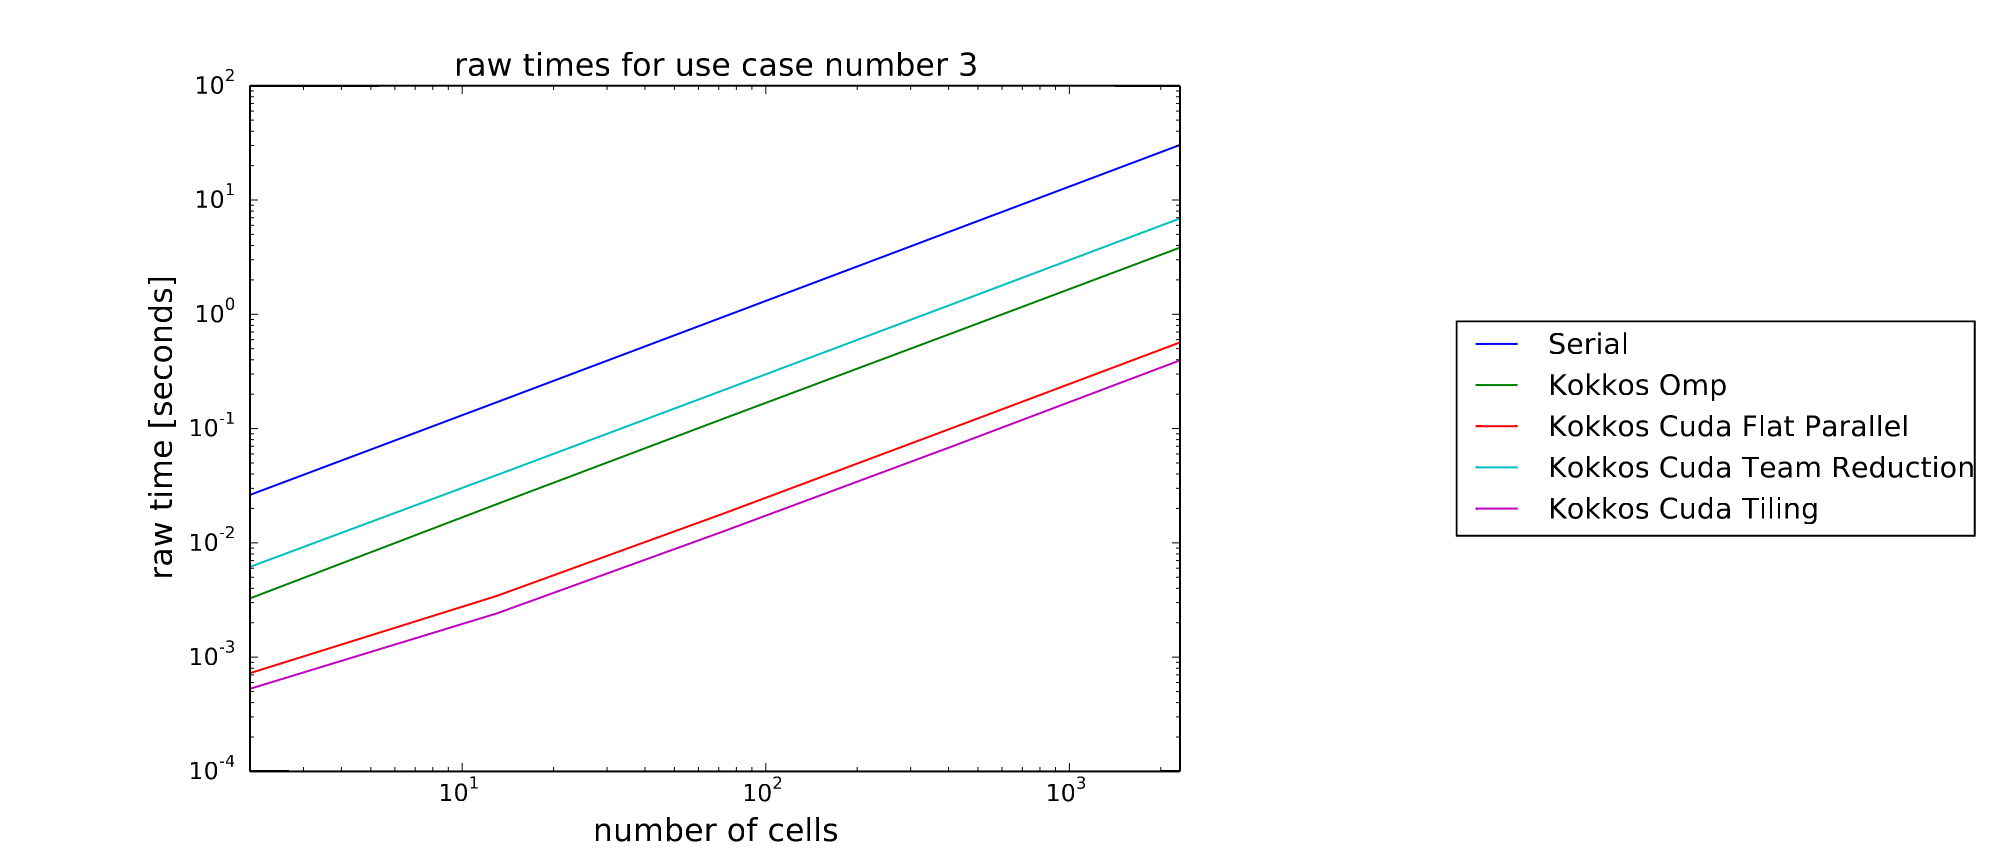
\includegraphics[scale = .2]{tilinguc1}
\caption{Raw times for many different algorithms used for ContractFieldFieldScalar. Note that Tiling is the best performing (lowest). This data was generated with $\ell=\mathcal{R}=125$, $p=216$}
\label{fig:TilingPerformance}
\end{figure}
Consider the graph generated in Figure~\ref{fig:TilingPerformance} for \texttt{ContractFieldFieldScalar}. We see that tiling outperforms both flat parallelism and team reductions across the board. This trend continues for smaller use cases as well, as shown in Figure~\ref{fig:TilingPerformance2} when $\ell = \mathcal{R} = 8$, $P = 8$.

\begin{figure}[H]
    \centering
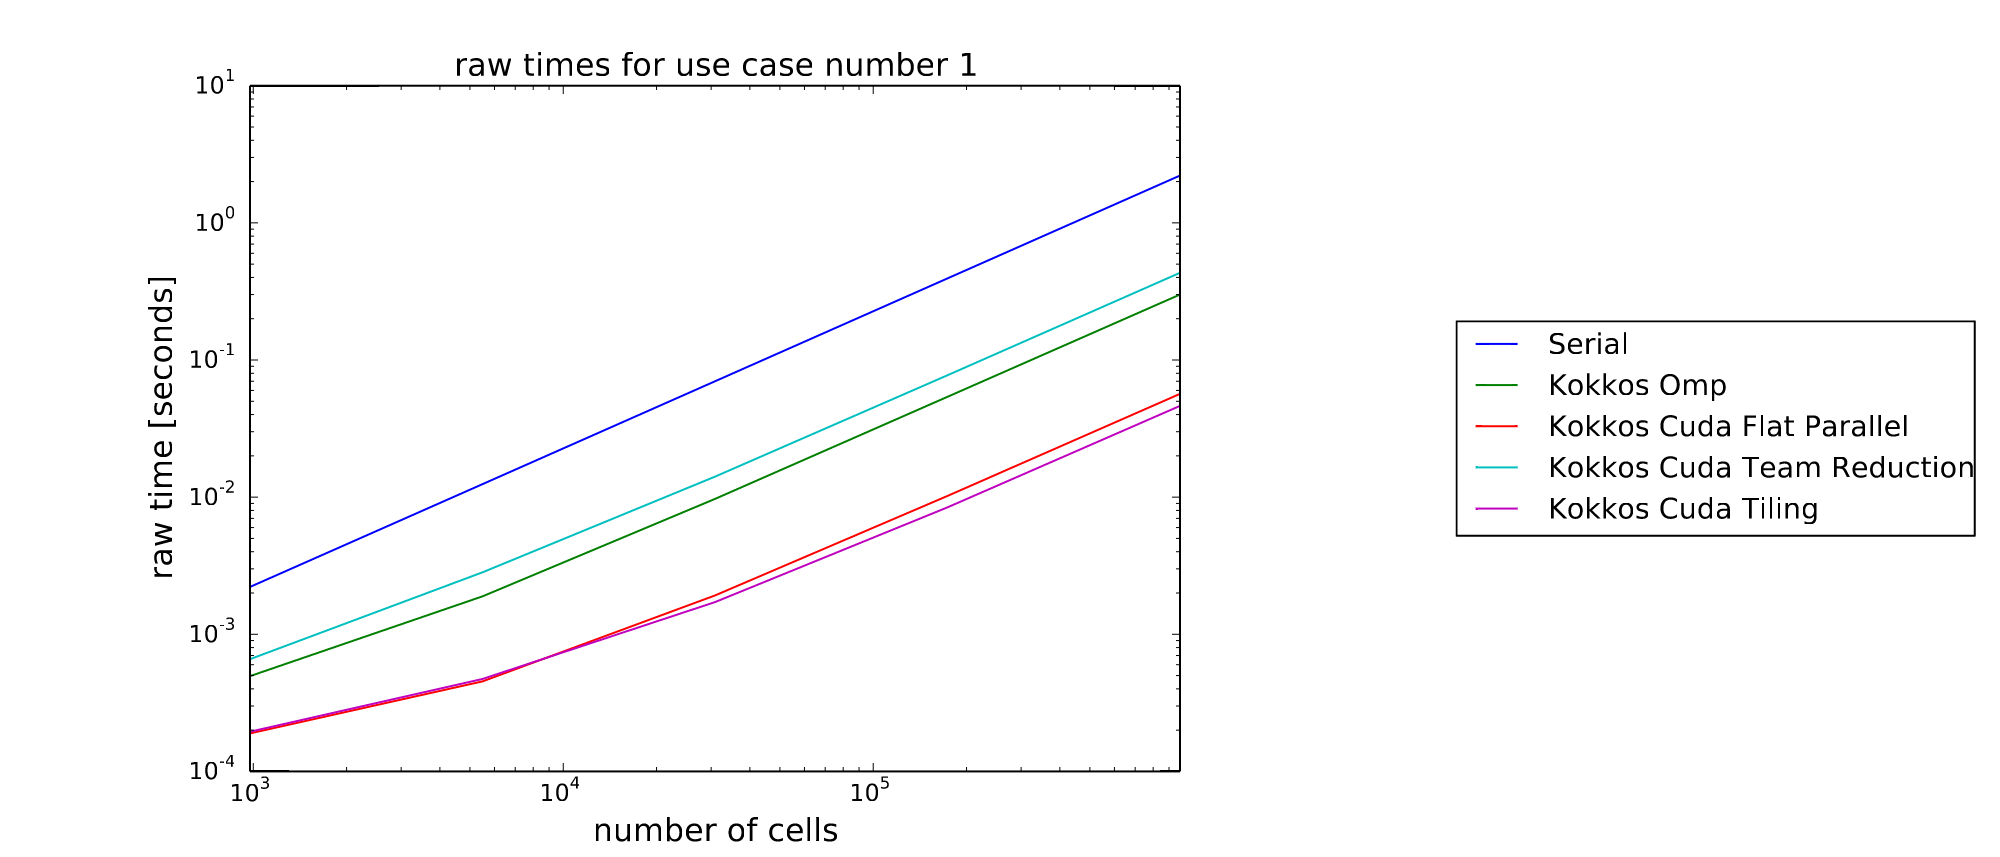
\includegraphics[scale = .2]{tilinguc2}
\caption{Raw times for many different algorithms used for ContractFieldFieldScalar. This data was generated with $\ell=\mathcal{R}=8$, $p=8$}
\label{fig:TilingPerformance2}
\end{figure}

\subsection{ContractFieldFieldTensor}

We also created a tiling implementation of \texttt{ContractFieldFieldTensor}. Conceptually, it is much more difficult to envision how to approach tiling on multidimensional problems. \texttt{ContractiFieldFieldTensor}, which can be described by the equation $L_{C,\ell,P,d_1,d_2} \times R_{C, \mathcal{R}, P,d_1,d_2} = O_{C,\ell, \mathcal{R}}$, therefore presents an interesting problem for the tiling approach. 

Unlike slicing, there seem to be multiple distinct ways of approaching the
problem. One can ``unroll" the entire contraction to create a situation where
the left and right matrices are rectangular, but can be covered by 2D tiles.
Alternatively, algorithms could cover the left and right inputs using
multidimentional tiles. While conceptually these two approaches seem distinct,
they are functionally equivalent. Ultimately, tiling involves loading pieces of
both the input and output matrices into shared memory and operating on them
repeatedly. As long as we avoid suboptimal memory access patterns, it makes no
difference whether we visualize the tiles as two dimensional or with even higher
dimensions. For ease of understanding, we implemented
\texttt{ContractFieldFieldTensor}'s tiling kernels with ``unrolled"
contractions. This essentially, reduces the kernel to a series of long dot
products in our vision of the memory layout. 

Using the tiling method on \texttt{ContractFieldFieldTensor} we were able to generate speedup of between $1.5$ and $2$ times over flat parallelism, as shown in Figure~\ref{fig:CFFTSpeedup}. 

\begin{figure}[H]
    \centering
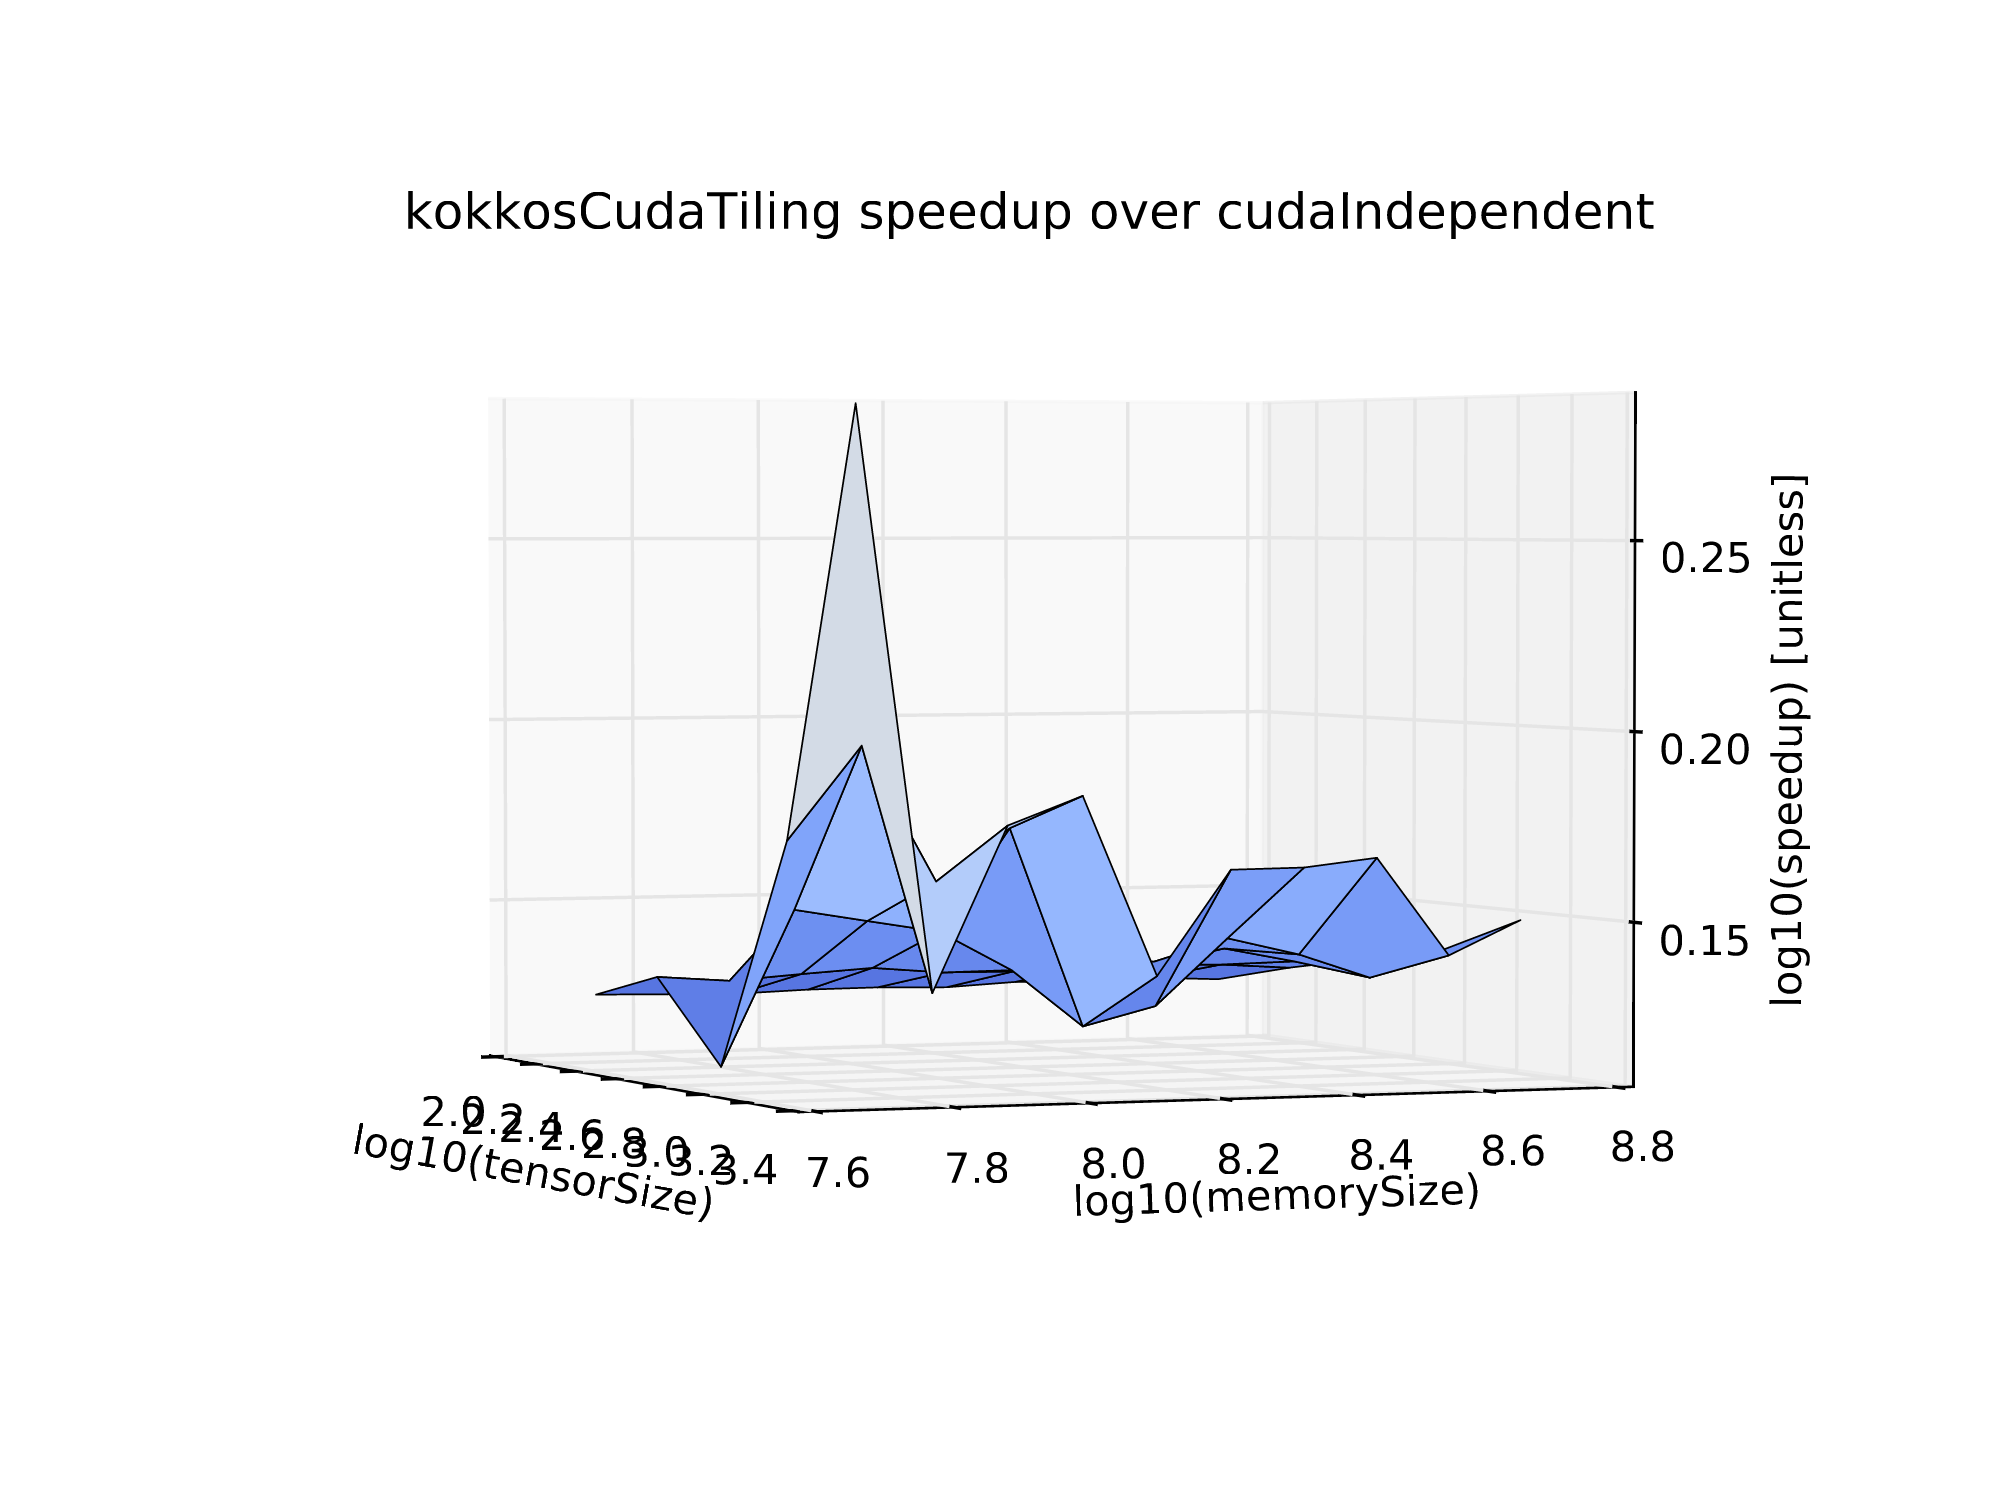
\includegraphics[scale = .2]{ContractFieldFieldTensor}
\caption{Speedup of Tiling for ContractFieldFieldTensor over independent parallelism. This data was generated with $\ell = \mathcal{R} = 16$, $d_1 = d_2 = 4$, and $P$ varying from 16 to 128.}
\label{fig:CFFTSpeedup}
\end{figure}

In these cases, the size of the contraction will often be larger than the number
of basis functions by as much as an order of magnitude. This makes tiling
significantly less efficient because the matrices are rectangular instead of
square, as we previously discussed. In this case, the number of GPU blocks
capable of working on a contraction using the tiling algorithm is given by
$\frac{\text{number of basis functions}}{\text{size of a tile}}$. While tiling
can still perform well in these use cases, as shown by
Figures~\ref{fig:multiDTiling1} and \ref{fig:multiDTiling2}, it does not perform
as well as on square matrices.

\begin{figure}[H]
    \centering
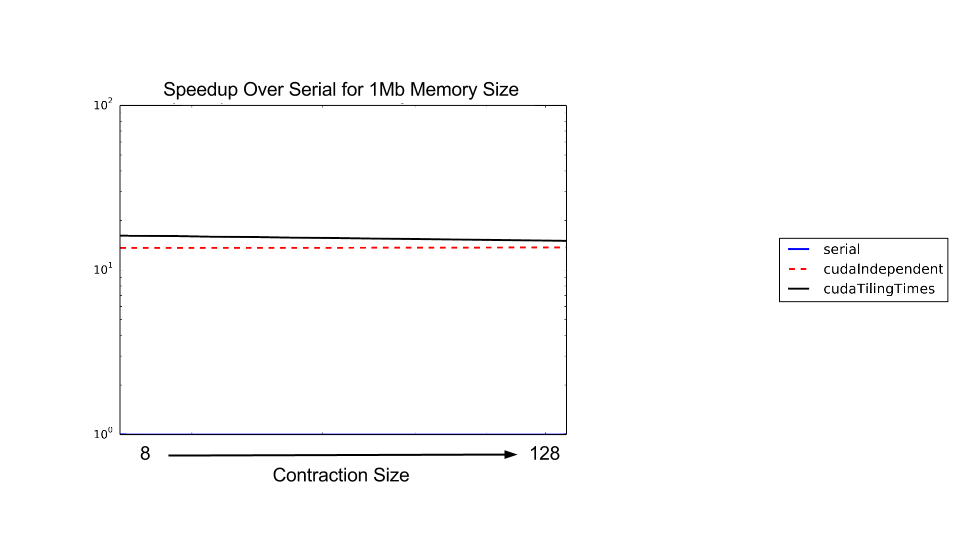
\includegraphics[scale = .2]{CFFTTiling1}
\caption{Raw times for serial, independent, and tiling approaches to \texttt{ContractFieldFieldScalar}. This data was generated with $\ell=\mathcal{R}=16$, $d_1=d_2=4$, with $p$ varying from $8$ to $128$. This graph uses a relatively low memory size, which limits the number of cells}
\label{fig:multiDTiling1}
\end{figure}

\begin{figure}[H]
    \centering
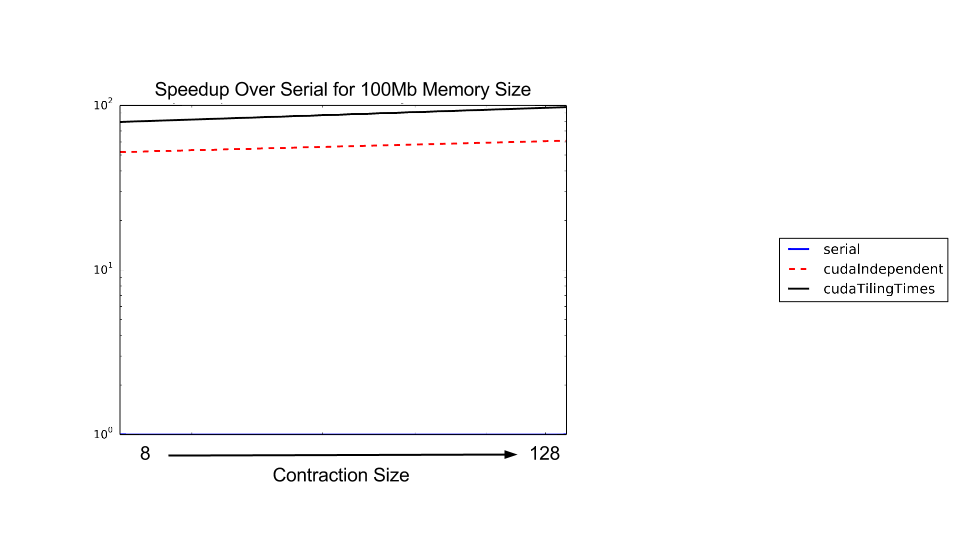
\includegraphics[scale = .2]{CFFTTiling2}
\caption{Raw times for serial, independent, and tiling approaches to \texttt{ContractFieldFieldScalar}. This data was generated with $\ell=\mathcal{R}=16$, $d_1=d_2=4$, with $p$ varying from $8$ to $128$. This data was collected while simulating a memory size an order of magnitude larger than the previous image, leading to a significantly higher cell count. }
\label{fig:multiDTiling2}
\end{figure}

Excerpts from our implementation of tiling for ContractFieldFieldTensor are included in Figure~\ref{lst:CFFTTiling}, which have been simplified using the assumption that $\ell=\mathcal{R}$ as well as the assumption that the size of each tile evenly divides every other dimension for clarity. 

\begin{figure}[H]
    \begin{lstlisting} [basicstyle=\tiny]

    // Here we pretend that all three contraction dimensions are a single dimension: contractionSize
    const unsigned int contractionSize = _dimTens1 * _dimTens2 * _numPoints;
    
    const unsigned int numberOfPointTiles = contractionSize / tile_size;
    const unsigned int numberOfBasisTiles = numBasis / tile_size;

    const unsigned int numberOfTiles = _numCells * numberOfBasisTiles * numberOfBasisTiles;
    
    //These are the subRow and subColumn of the thread within its tile
    const unsigned int subRow = thread.team_rank() / _tile_size;
    const unsigned int subCol = thread.team_rank() - subRow * _tile_size;

    unsigned int resultTileIndex = thread.league_rank();
    //Our shared memory for the computation, which fits two full tiles
    Kokkos::View<float*, Kokkos::MemoryUnmanaged> tileStorage(thread.team_shmem(), 2 * _tile_size * _tile_size);

    const unsigned int resultMatrix = resultTileIndex / (numberOfBasisTiles * numberOfBasisTiles);
    const unsigned int resultSubmatrixIndex = resultTileIndex - (resultMatrix * numberOfBasisTiles * numberOfBasisTiles); // (mod)

    // calculate result tile indices
    const unsigned int resultTileRow = resultSubmatrixIndex / numberOfBasisTiles;
    const unsigned int resultTileCol = resultSubmatrixIndex - resultTileRow * numberOfBasisTiles; // (mod)

    // calculate this threads actual output index
    const unsigned int row = resultTileRow * _tile_size + subRow;
    const unsigned int col = resultTileCol * _tile_size + subCol;
    float sum = 0;

    // for tileNumber in 0...numberOfTilesPerSide
    for (unsigned int tileNumber = 0; tileNumber < numberOfPointTiles; ++tileNumber) {

        // these are base indices into the shared memory
        const unsigned int leftBaseIndex = subRow * _tile_size;
        const unsigned int rightBaseIndex = _tile_size*_tile_size + subCol;

        // Here we break it back down so that we can use it
        const unsigned int leftContractionIndex = tileNumber*_tile_size + subCol;
        const unsigned int left_qp = leftContractionIndex / (_dimTens1*_dimTens2);
        const unsigned int left_combinedTens = leftContractionIndex - left_qp * (_dimTens1 * _dimTens2); // (mod)
        const unsigned int left_iTens1 = left_combinedTens / _dimTens2;
        const unsigned int left_iTens2 = left_combinedTens - left_iTens1 * _dimTens2; // (mod)

        const unsigned int rightContractionIndex = tileNumber * _tile_size + subRow; 
        const unsigned int right_qp = rightContractionIndex / (_dimTens1*_dimTens2);
        const unsigned int right_combinedTens = rightContractionIndex - right_qp * (_dimTens1 * _dimTens2); // (mod)
        const unsigned int right_iTens1 = right_combinedTens / _dimTens2;
        const unsigned int right_iTens2 = right_combinedTens - right_iTens1 * _dimTens2; // (mod)

        // load the left and right tiles into shared memory
        tileStorage(thread.team_rank()) = _leftView(resultMatrix, row, left_qp, left_iTens1, left_iTens2);
        tileStorage(thread.team_rank() + (_tile_size * _tile_size)) =
            _rightView(resultMatrix, right_qp, right_iTens1, right_iTens2, col);

        // make sure everyone's finished loading their pieces of the tiles
        thread.team_barrier();

        for (unsigned int dummy = 0; dummy < _tile_size; ++dummy) {
          sum +=
            tileStorage(leftBaseIndex + dummy) *
            tileStorage(rightBaseIndex + dummy * _tile_size);
        }
        thread.team_barrier();
      }
      
      _outputView(resultMatrix, row, col) = sum;
      
 \end{lstlisting}
 \caption{Something should be here} %TODO
\label{lst:CFFTTiling}
\end{figure}
 
 
